% Native PGFPlots; generated by examples/generate_figures.py.
% Constructed or analytical teaching example.
\begingroup
\definecolor{blueplot}{HTML}{4E79A7}
\definecolor{redplot}{HTML}{D95F59}
\definecolor{inkplot}{HTML}{111111}
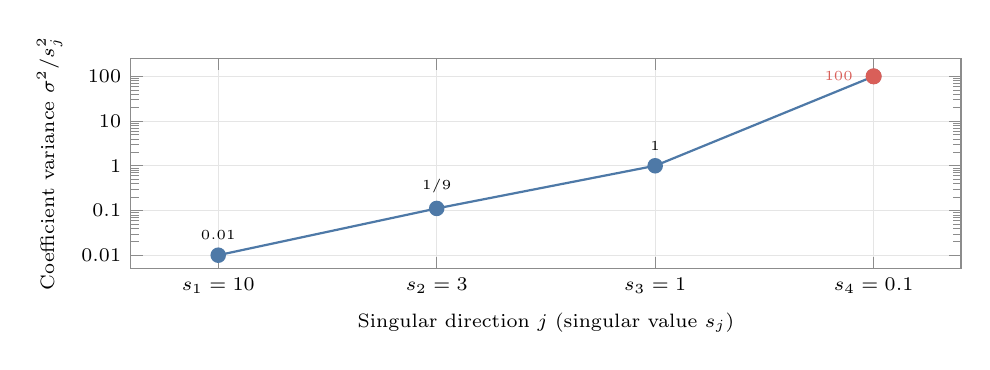
\begin{tikzpicture}
\begin{axis}[
width=\linewidth,height=4.25cm,font=\scriptsize,
tick label style={font=\scriptsize},label style={font=\scriptsize},
axis line style={black!45},tick style={black!45},
grid=major,grid style={black!10},scaled ticks=false,
clip=true,unbounded coords=jump,
legend style={font=\tiny,draw=none,fill=white,fill opacity=.94,text opacity=1,
  legend cell align=left,inner sep=2pt,row sep=1pt},
xmin=.6,xmax=4.4,ymin=.005,ymax=250,
xlabel={Singular direction $j$ (singular value $s_j$)},
ylabel={Coefficient variance $\sigma^2/s_j^2$},
xtick={1,2,3,4},xticklabels={$s_1=10$,$s_2=3$,$s_3=1$,$s_4=0.1$},
ymode=log,ytick={.01,.1,1,10,100},log ticks with fixed point,
]
\addplot[blueplot,thick,mark=*,mark size=2.4pt] coordinates {(1,.01) (2,.1111111111) (3,1) (4,100)};
\node[font=\tiny,anchor=south,yshift=2pt] at (axis cs:1,.01) {$0.01$};
\node[font=\tiny,anchor=south,yshift=2pt] at (axis cs:2,.1111111111) {$1/9$};
\node[font=\tiny,anchor=south,yshift=2pt] at (axis cs:3,1) {$1$};
\node[font=\tiny,anchor=east,xshift=-4pt,text=redplot] at (axis cs:4,100) {$100$};
\addplot[only marks,redplot,mark=*,mark size=2.7pt] coordinates {(4,100)};

\end{axis}
\end{tikzpicture}
\endgroup
